\documentclass[11pt]{article}
\usepackage{graphicx}
\usepackage[authoryear,round]{natbib}
\usepackage{caption}
\usepackage{subcaption}
\usepackage[mathlines]{lineno}
\usepackage{setspace}
\usepackage{mathrsfs}
\usepackage{rotating}
\usepackage{url}
\usepackage{amssymb}
\usepackage{multirow}
\usepackage[none]{hyphenat}
\usepackage{algpseudocode}
\DeclareGraphicsExtensions{.pdf,.png,.jpg}
\setlength{\topmargin}{-0.5in}
\setlength{\textheight}{10in}
\setlength{\oddsidemargin}{.125in}
\setlength{\textwidth}{6.25in}
\doublespacing
\pagestyle{empty}

\captionsetup[subfigure]{labelfont=rm}

\begin{document}

\begin{figure}[h!]
   \centering
   \begin{subfigure}[b]{0.49\textwidth}
    \centering
   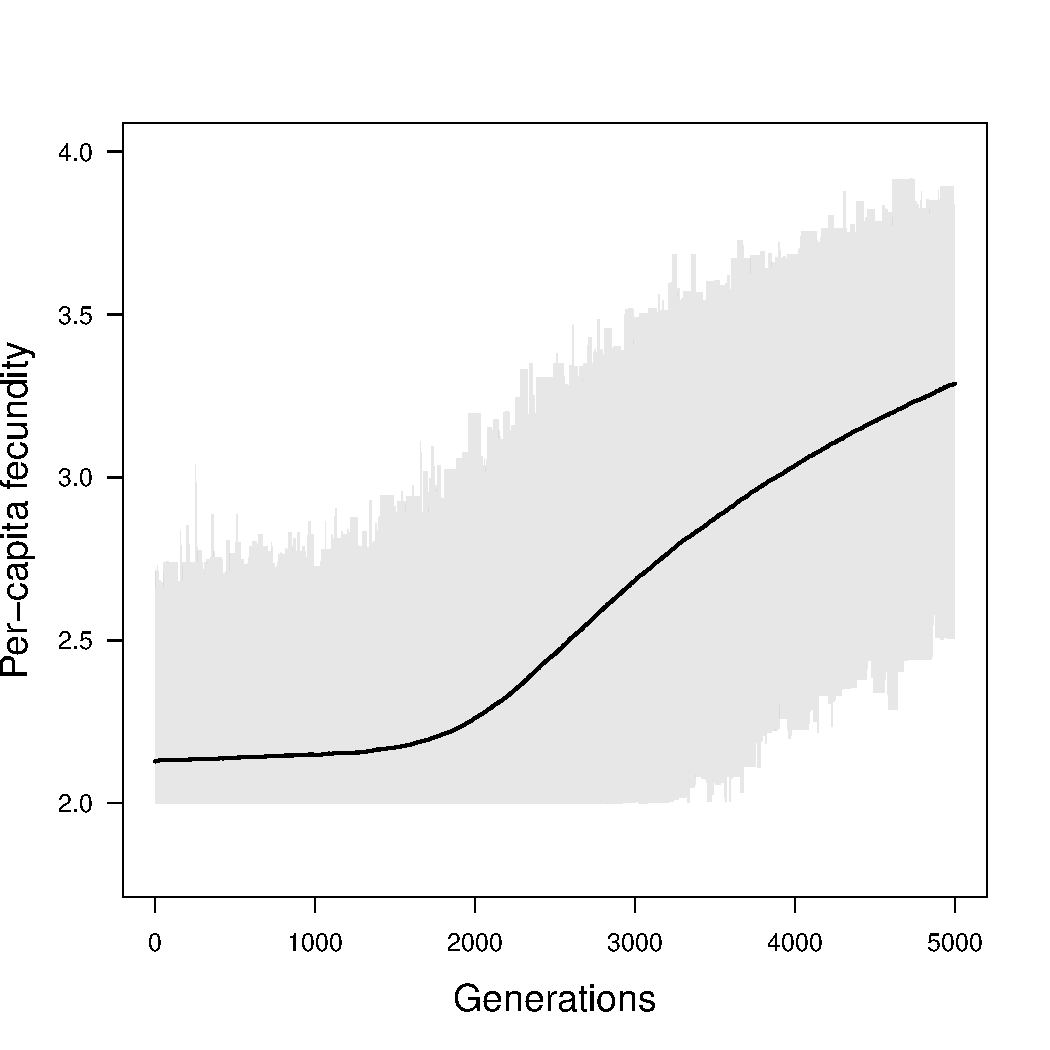
\includegraphics[width=\linewidth] {SupplementaryFigures/FigS1A.pdf}\quad
	\caption*{(A)}        
	\end{subfigure}
   \begin{subfigure}[b]{0.49\textwidth}
    \centering
   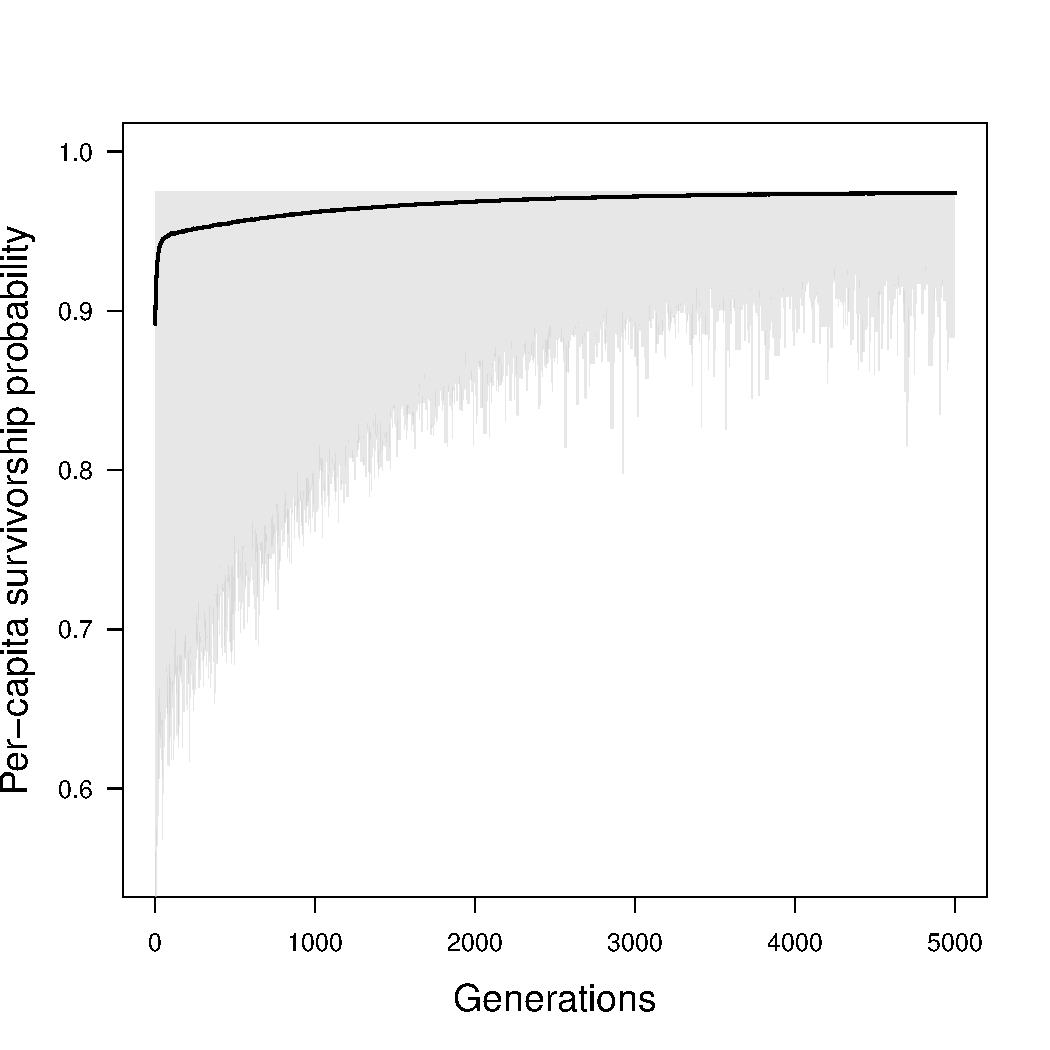
\includegraphics[width=\linewidth] {SupplementaryFigures/FigS1B.pdf}
	\caption*{(B)}
  	\end{subfigure}
\caption*{Figure S1. The evolutionary trajectory of the average traits determining per-capita fecundity (A) and the per-time step per-capita survivorship probability (B). To prevent individuals from living forever (i.e., to have a survivorship probability of one), the maximum evolvable per-time step survivorship has an asymptote at 0.975, which corresponds to an average lifespan of approximately 40 time steps. In each panel, the grey region represents the maximum and minimum trait values in each deme. For further details, see the main text.}

\end{figure}
\end{document}

